% !TeX root = ../Doc_especific_mse_anchovy.tex

\begin{figure}[h]
    \centering
    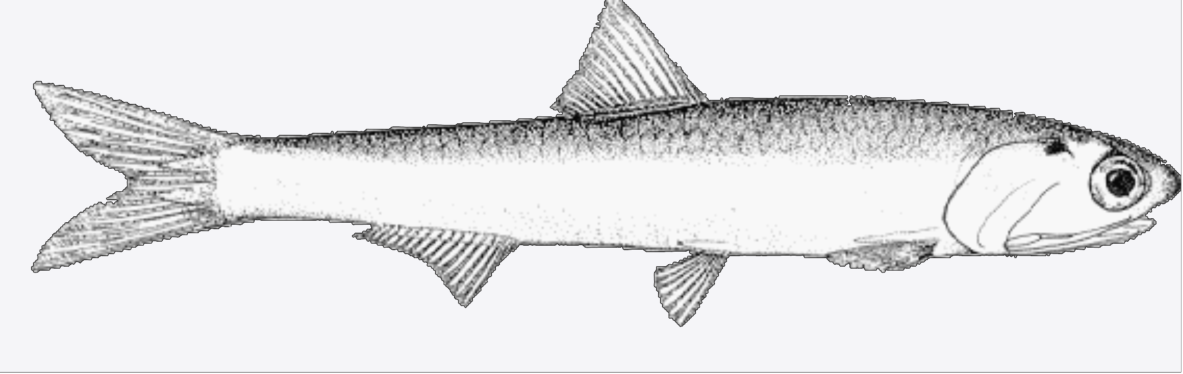
\includegraphics[scale=0.4]{figura1.pdf}  
    \caption{Anchoveta Engraulis ringens (Jenyns 1842).}
    \label{fig:figure1}
\end{figure}  

Engraulis ringens es una especie pelágica (Figura 1) que se distribuye principalmente entre los 4$^\circ$ LS hasta los 42$^\circ$ LS, distinguiéndose tres stocks; uno que va desde el norte y centro del Perú, otro que va desde el sur del Perú al norte de Chile y el último en la zona central de Chile (Claramunt et al., 2012). Para este estudio, el área de distribución de la anchoveta está entre el sur de Perú y norte de Chile (16$^\circ$LS – 24$^\circ$LS, Figura 2) en la cual la especie constituye una unidad stock independiente del norte-centro de Perú, norte-centro y centro-sur de Chile, siendo una unidad de stock y pesquería independiente (Cubillos et al., 2007).
\newline

Es importante señalar que el stock de anchoveta del sur de Perú y norte de Chile se plantea como un stock independiente del stock de anchoveta de la III y IV región (Leal y Canales, 2014). Canales y Leal (2009) plantean que la anchoveta centro-norte podría corresponder a una unidad poblacional independiente de la ubicada al norte de los 25$^\circ$ LS, que recluta, crece y se reproduce en el área. Los cruceros oceanográficos desarrollados en la década de 1980 muestran focos discretos de desove (huevos y larvas) de anchoveta en las bahías de Caldera y Coquimbo (Rojas et al., 1983). Esto sugiere que la zona centro-norte de Chile podría representar un hábitat favorable para la anchoveta particularmente en las bahías de Caldera y Coquimbo, donde existen patrones de circulación y focos de surgencia (Valle-Levinson y Moraga, 2006) que podrían facilitar la retención y desarrollo de la anchoveta en estas bahías. Serra y Gil (1975) estudiaron la migración del stock de la anchoveta del sur de Perú y norte de Chile mostrando la ocurrencia de intensos y amplios movimientos migratorios hacia el sur de Perú en invierno y verano. Menos intensos y amplios son los movimientos migratorios de anchoveta con dirección hacia los 24$^\circ$ LS. Un estudio similar fue realizado por Martínez et al. (1998) reportaron resultados similares en términos de dirección e intensidad de las migraciones. Se plantea que en la zona comprendida entre los 24$^\circ$ LS y 25$^\circ$ LS al parecer no existirían las condiciones oceanográficas para permitir un flujo continuo que permita la residencia de focos anchoveta entre ambas zonas (Serra, com. pers.). Las poblaciones de Caldera y Coquimbo habrían surgido cuando en algunos años (y por razones ambientales, e.i. El Niño), la anchoveta de la zona norte expande su distribución hacia el sur de los 24$^\circ$ LS, colonizando las bahías de Caldera y Coquimbo donde procesos oceanográficos permiten el crecimiento y desarrollo de la anchoveta. Sin embargo, esta hipótesis no ha sido demostrada aún.

\begin{figure}[H]
    \centering
    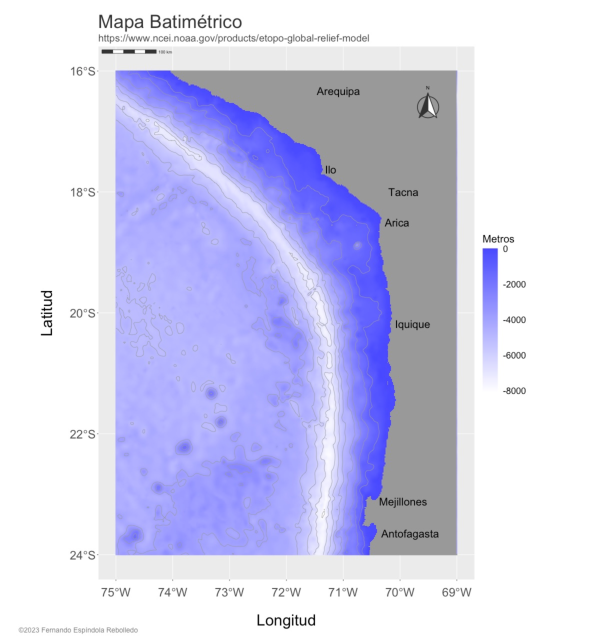
\includegraphics[scale=1.1]{figura2.pdf}  
    \caption{Área de distribución del stock de anchoveta del sur de Perú y norte de Chile, distribuido entre los 16$^\circ$ LS – 24$^\circ$ LS (FUENTE: Modelo Global de Elevación Batimétrico, ETOPO1-NOAA).}
    \label{fig:figure2}
\end{figure}  